\begin{theorem}[\textbf{Teorema de Stokes}]
Sea $D \subset \mathbb{R}^2$ un conjunto compacto cuya frontera $\partial D$ está formada por un número finito de curvas cerradas simples y suaves por trozos. Sea $\boldsymbol{\Sigma}: D \to \mathbb{R}^3$ una parametrización continua en $D$, regular y de clase $\mathcal{C}^1(\interior{D})$, que define una superficie $S = \boldsymbol{\Sigma}(D)$  cuyo borde geométrico está dado por $\partial S = \boldsymbol{\Sigma}(\partial D)$. 

Sea $A \subseteq \mathbb{R}^3$ un conjunto abierto tal que $S \subset A$. Si $\mathbf{F}: A \to \mathbb{R}^3$ es un campo vectorial de clase $\mathcal{C}^1(A)$, entonces:
\[
\oint_{\partial S}\mathbf{F}\cdot d\mathbf{s} = \iint_S (\nabla \times \mathbf{F})\cdot d\mathbf{S}, 
\]
donde las orientaciones tanto de $S$ como de $\partial S$ son las inducidas por $\boldsymbol{\Sigma}$ sobre ellas, ver (\ref{sigma_induce_1}) y (\ref{sigma_induce}).
\end{theorem}



\begin{example} Verificar el Teorema de Stokes para el campo vectorial $\mathbf{F} = (x^2y, 3x^3z, yz^3)$ y la superficie $S$ dada por el cilindro $x^2 + y^2 = 1$ con $-1 \le z \le 1$ con orintaci\'on $n$  ``saliente"  del cilindro. 
\end{example} \noindent\textbf{Solución:} dibujemos la superficie dada 



\begin{figure}[h]
    \centering
    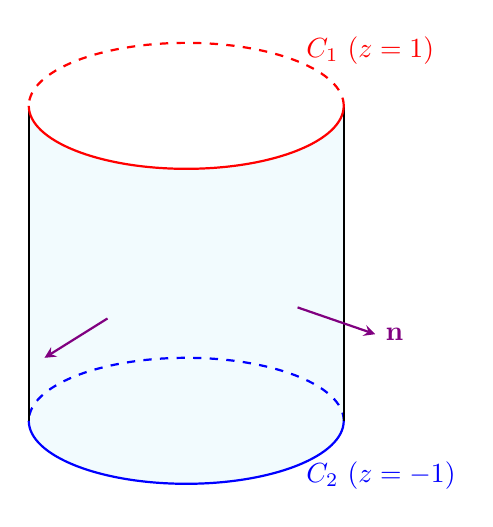
\begin{tikzpicture}[scale=2, >=stealth]
        % 1. SUPERFICIE DEL CILINDRO (Fondo coloreado cian)
        \fill[cyan!10, opacity=0.5] (-1,-1) -- (-1,1) arc (180:360:1 and 0.4) -- (1,-1) arc (360:180:1 and 0.4);
        
        % 2. MITAD TRASERA OCULTA DE LAS TAPAS (Punteadas con el color correspondiente)
        \draw[dashed, red, thick] (1,1) arc (0:180:1 and 0.4);
        \draw[dashed, blue, thick] (1,-1) arc (0:180:1 and 0.4);
    
        % 3. LÍNEAS VERTICALES DE CONTORNO (Generatrices del cilindro)
        \draw[thick] (-1,-1) -- (-1,1);
        \draw[thick] (1,-1) -- (1,1);
    
        % 4. CURVA SUPERIOR C1 (z = 1) - MITAD DELANTERA VISIBLE (Roja)
        \draw[thick, red] (-1,1) arc (180:360:1 and 0.4);
      %  \draw[thick, red, ->] (-1,1) arc (180:240:1 and 0.4);
       % \draw[thick, red, ->] (0,0.6) arc (-90:-30:1 and 0.4);
        \node[red, above right] at (0.7, 1.2) {$C_1\ (z=1)$};
    
        % 5. CURVA INFERIOR C2 (z = -1) - MITAD DELANTERA VISIBLE (Azul)
        \draw[thick, blue] (-1,-1) arc (180:360:1 and 0.4);
       % \draw[thick, blue, ->] (1,-1) arc (0:-60:1 and 0.4);
        % \draw[thick, blue, ->] (0,-1.4) arc (-90:-150:1 and 0.4);
        \node[blue, below right] at (0.7,-1.2) {$C_2 \ (z=-1)$};
    
        % 6. VECTORES NORMALES SALIENTES (n)
        \draw[->, thick, violet] (0.707, -0.28) -- (1.2, -0.45) node[right] {$\mathbf{n}$};
        \draw[->, thick, violet] (-0.5, -0.35) -- (-0.9, -0.6);
    \end{tikzpicture}
    \caption{Representación geométrica del cilindro $S$ con orientación saliente $\mathbf{n}$. }
\label{fig:cilindro_stokes}
\end{figure}  Para verificar el teorema, podemos utilizar un argumento topológico análogo al empleado en la generalización del Teorema de Green. Dividimos la superficie del cilindro $S$ mediante dos cortes verticales en dos subsuperficies, $S_1$ y $S_2$, de modo que el borde geométrico de cada una sea una única curva cerrada simple.  





\begin{figure}[h]
    \centering
    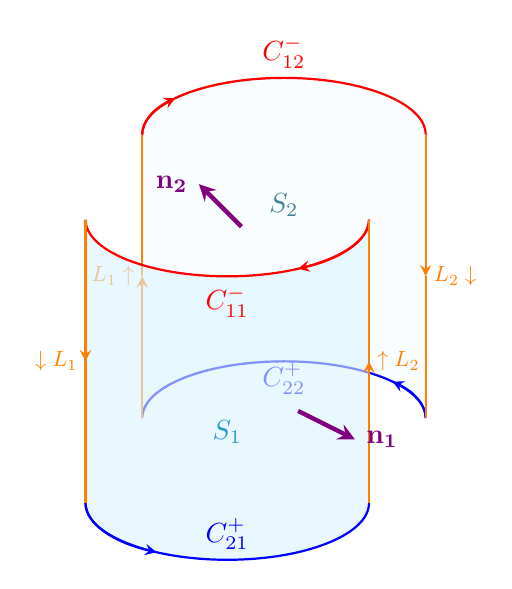
\begin{tikzpicture}[scale=1.8, >=stealth]
        
        % ==========================================
        % 1. MITAD TRASERA (S_2) - Desplazada levemente hacia atrás/arriba
        % ==========================================
        \begin{scope}[shift={(0.2,0.3)}]
            % Fondo coloreado S2
            \fill[cyan!5, opacity=0.4] (-1,-1) -- (-1,1) arc (180:0:1 and 0.4) -- (1,-1) arc (0:180:1 and 0.4);
            
            % Arcos traseros de las tapas (Ocultos reales)
            \draw[dashed, color=red!40, thick] (0,1.4) arc (90:180:1 and 0.4);
            \draw[dashed, color=blue!40, thick] (0,-0.6) arc (90:180:1 and 0.4);
            
            % Arcos delanteros de S2 (que forman su contorno interior)
            \draw[thick, red] (-1,1) arc (180:0:1 and 0.4);
            \draw[thick, blue] (-1,-1) arc (180:0:1 and 0.4);
            
            % Frontera S2 orientada para normal exterior (n2 hacia atrás, giro horario visto desde atrás = antihorario visto de frente)
            % Tapa superior trasera (flecha hacia la derecha)
            \draw[thick, red, ->] (-1,1) arc (180:140:1 and 0.4);
            \node[red, above] at (0,1.4) {$C_{12}^{-}$};
            
            % Tapa inferior trasera (flecha hacia la izquierda)
            \draw[thick, blue, ->] (1,-1) arc (0:40:1 and 0.4);
           \node[blue, above] at (0,-0.9) {$C_{22}^{+}$};
            
            % Cortes verticales para S2 (Naranja de cancelación)
            \draw[thick, orange, ->] (-1,-1) -- (-1,0) node[left, scale=0.8] {$L_1 \uparrow$};
            \draw[thick, orange] (-1,0) -- (-1,1);
            
            \draw[thick, orange, ->] (1,1) -- (1,0) node[right, scale=0.8] {$L_2 \downarrow$};
            \draw[thick, orange] (1,0) -- (1,-1);
            
            % Etiqueta de la superficie trasera
            \node[cyan!60!black] at (0,0.5) {$S_2$};

            % Vector normal saliente en S2
            \draw[->, ultra thick, violet] (-0.3,0.35) -- (-0.6,0.65) node[left] {$\mathbf{n_2}$};
        \end{scope}
       

        % ==========================================
        % 2. MITAD DELANTERA (S_1) - En la posición original
        % ==========================================
        \begin{scope}[shift={(-0.2,-0.3)}]
            % Fondo coloreado S1
            \fill[cyan!15, opacity=0.6] (-1,-1) -- (-1,1) arc (180:360:1 and 0.4) -- (1,-1) arc (360:180:1 and 0.4);
            
            % Contornos laterales del cilindro delantero
            \draw[thick, gray!80] (-1,-1) -- (-1,1);
            \draw[thick, gray!80] (1,-1) -- (1,1);
            
            % Arcos delanteros visibles de S1
            \draw[thick, red] (-1,1) arc (180:360:1 and 0.4);
            \draw[thick, blue] (-1,-1) arc (180:360:1 and 0.4);
            
            % Frontera S1 orientada para normal exterior (n1 hacia adelante, giro antihorario en pantalla)
            % Tapa superior delantera (flecha hacia la izquierda, horario visto desde arriba)
            \draw[thick, red, ->] (1,1) arc (360:300:1 and 0.4);
            \node[red, below] at (0,0.6) {$C_{11}^{-}$};
            
            % Tapa inferior delantera (flecha hacia la derecha, antihorario visto desde arriba)
            \draw[thick, blue, ->] (-1,-1) arc (180:240:1 and 0.4);
            \node[blue, above] at (0,-1.4) {$C_{21}^{+}$};
            
            % Cortes verticales para S1 (Sentidos opuestos a S2)
            \draw[thick, orange, ->] (-1,1) -- (-1,0) node[left, scale=0.8] {$\downarrow L_1$};
            \draw[thick, orange] (-1,0) -- (-1,-1);
            
            \draw[thick, orange, ->] (1,-1) -- (1,0) node[right, scale=0.8] {$\uparrow L_2$};
            \draw[thick, orange] (1,0) -- (1,1);
            
            % Etiqueta de la superficie delantera
            \node[cyan!80!black] at (0,-0.5) {$S_1$};
            
            % Vector normal saliente en S1
            \draw[->, ultra thick, violet] (0.5,-0.35) -- (0.9,-0.55) node[right] {$\mathbf{n_1}$};
        \end{scope}

    \end{tikzpicture}
    \caption{Descomposición del cilindro $S$ en dos subsuperficies simplemente conexas $S_1$ y $S_2$. Las líneas de corte verticales $L_1$ y $L_2$ se recorren en sentidos opuestos.}
\label{fig:cilindro_stokes_1}
\end{figure}







Las curvas $C_1$ y $C_2$ se definen formalmente en $\mathbb{R}^3$ como la intersección de la superficie cilíndrica con los planos $z = 1$ y $z = -1$ respectivamente, es decir:
\begin{align*}
C_1 &= \left\{ (x, y, z) \in \mathbb{R}^3 : x^2 + y^2 = 1, \; z = 1 \right\} \\[1ex]
C_2 &= \left\{ (x, y, z) \in \mathbb{R}^3 : x^2 + y^2 = 1, \; z = -1 \right\}
\end{align*}

Tal como muetra la Figura \ref{fig:cilindro_stokes_1} , las curvas $C_1$ y $C_2$  pueden ser escritas, junto con una  orientaci\'on,  como:   $$ C_1^{-} = C_{11}^{-} \cup  C_{12}^{-} \quad  \text{ y } \quad   C_2^{+} = C_{21}^{+} \cup C_{22}^{+}$$  

Al aplicar el Teorema de Stokes en cada superficie $S_1$ y $S_2$  por separado, sumar los resultados y considerando que las integrales de línea a lo largo de los cortes verticales $L_1$ y  $L_2$   se recorren en sentidos opuestos, estas se cancelan mutuamente,  obtenemos:
\begin{align*}
\iint_{S} (\nabla \times \mathbf{F}) \cdot \mathbf{n}\, dS &= \iint_{S_1} (\nabla \times \mathbf{F}) \cdot \mathbf{n_1}\, dS + \iint_{S_2} (\nabla \times \mathbf{F}) \cdot \mathbf{n_2}\, dS \\[1ex]
&= \oint_{\partial S_1^{-}} \mathbf{F} \cdot d\mathbf{s} + \oint_{\partial S_2^{+}} \mathbf{F} \cdot d\mathbf{s} \\[1ex]
&= \oint_{C_1^{-}} \mathbf{F} \cdot d\mathbf{s} + \oint_{C_2^{+}} \mathbf{F} \cdot d\mathbf{s}
\end{align*}
con  $$ \partial S_1^{-} = C_{11}^{-} \cup L_1^{-}  \cup   C_{21}^{+}   \cup  L_2^{+} $$ y $$ \partial S_2^{+} = C_{12}^{-} \cup L_2^{-}  \cup   C_{22}^{+}   \cup  L_1^{+} $$  
donde las orientaciones correspondientes son mostradas en la Figura  \ref{fig:cilindro_stokes_1}.  

Calculemos primero $\iint_{S} (\nabla \times \mathbf{F}) \cdot \mathbf{n}\, dS$.   El rotor del campo vectorial $\mathbf{F}$ está dado por: 
\[
\nabla \times \mathbf{F}(x,y,z) = (z^3 - 3x^3, 0, 9x^2z - x^2)
\]
Parametrizamos el cilindro utilizando coordenadas cilíndricas:  
\[
\boldsymbol{\Sigma}(\theta, z) = (\cos\theta, \sin\theta, z) \quad \text{con } 0 \le \theta \le 2\pi, \; -1 \le z \le 1
\]
Las derivadas parciales y su producto vectorial resultan en:
\begin{align*}
\boldsymbol{\Sigma}_{\theta}(\theta, z) &= (-\sin\theta, \cos\theta, 0) \\
\boldsymbol{\Sigma}_z (\theta, z) &= (0, 0, 1) \\
\boldsymbol{\Sigma}_{\theta} \times \boldsymbol{\Sigma}_z (\theta, z) &= (\cos\theta, \sin\theta, 0)
\end{align*}
Se observa que este vector normal apunta hacia afuera del cilindro, respetando la orientación  ``saliente"  requerida. 

Luego, calculamos el producto escalar con el rotor evaluado en la superficie, obteniendo:
\[
(\nabla \times \mathbf{F})\circ (\boldsymbol{\Sigma}(\theta, z)) \cdot (\boldsymbol{\Sigma}_{\theta} \times \boldsymbol{\Sigma}_z)(\theta, z) = z^3\cos\theta - 3\cos^4\theta
\]
Por lo tanto, la integral de superficie buscada se reduce a:
\begin{align*}
\iint_{S} (\nabla \times \mathbf{F}) \cdot \mathbf{n}\, dS &= \int_{-1}^{1} \int_{0}^{2\pi} (z^3\cos\theta - 3\cos^4\theta) \, d\theta \, dz \\
&= \int_{-1}^{1} \left( 0 - 3 \cdot \frac{3\pi}{4} \right) dz \\
&= -\frac{9\pi}{4} \int_{-1}^{1} dz = -\frac{9\pi}{2}
\end{align*}





La parametrización de la curva \(C_{1}\) se define formalmente mediante$$ \sigma_1(\theta) = (\cos\theta, \sin\theta, 1) \mbox{ con }  \theta \in [ 0,2\pi], $$ y  $$\sigma'_1(\theta) = (-\sin\theta, \cos\theta, 0).$$

Observando que la parametrizaci\'on  elegida $ \sigma_1$ invienrte la orientaci\'on de la curva $ C_1$, la integral de línea  queda  $$ \oint_{C_1^{-}} \mathbf{F} \cdot d\mathbf{s} =  -\int_{0}^{2\pi} (-\cos^2\theta\sin^2\theta + 3\cos^4\theta) \, d\theta$$.

\smallskip
Analogamente,  la parametrización de la curva \(C_{2}\) se define formalmente mediante \[ \sigma_2(\theta) = (\cos\theta, \sin\theta, -1) \text{ con }  \theta \in  [ 0,2\pi], \] y   
\[\sigma'_2(\theta) = (-\sin\theta, \cos\theta, 0).\] 
	
Observando que la parametrizaci\'on  elegida $ \sigma_2$ preserva la orientaci\'on de la curva $ C_2$, la integral de línea  queda  \[ \oint_{C^{+}_2} \mathbf{F} \cdot d\mathbf{s} =  \int_{0}^{2\pi} (-\cos^2\theta\sin^2\theta - 3\cos^4\theta) \, d\theta \].

\smallskip
Luego, sumando ambas contribuciones para obtener la integral sobre toda la frontera:
\begin{align*}
\oint_{\partial S} \mathbf{F} \cdot d\mathbf{s} &= \int_{0}^{2\pi} (\cos^2\theta\sin^2\theta - 3\cos^4\theta) \, d\theta +  \int_{0}^{2\pi} (-\cos^2\theta\sin^2\theta - 3\cos^4\theta) \, d\theta \\[1ex]
&= \int_{0}^{2\pi} -6\cos^4\theta \, d\theta = -\frac{9\pi}{2}. 
\end{align*} Por lo tanto hemos verificado el **Teorema de Stokes**.




\begin{tarea} Sean  $S=\{  (x,y,z) \in \mathbb{R}^{3} \: : \:  x ^{2}+ y^{2} = z,  x ^{2}+ y^{2}  \leq 4 \}$  y $F(x,y,z) = (x ^{2}z^{2}, y^{2}z^{2}, xyz)$, calcular, indicando la orientaci\'on elegida   $$\iint_S\grad\times\mathbf{F}\cdot d\mathbf{S}$$
\end{tarea}

\begin{tarea} Sea  $C=\{  (x,y,z) \in \mathbb{R}^{3} \: : \:  z=4, \: x ^{2}+ y^{2}   = 4 \}$  una curva cerrada y simple y sea  $F(x,y,z) = (x ^{3}z^{3}+y, y^{\frac{1}{3}}z^{2}, xyz)$,  calcular,  indicando la orientaci\'on elegida,      $$\int_{C}\mathbf{F}\cdot d\mathbf{S}$$
\end{tarea}